% !TeX program = xelatex
% !TeX program = xelatex
% ===========================================================================
%  tech_common.tex -- 两份技术文档共用的导言区
% ===========================================================================
\documentclass[11pt,a4paper]{ctexart}

\usepackage[top=2.4cm,bottom=2.4cm,left=2.4cm,right=2.4cm]{geometry}
\usepackage{amsmath,amssymb,amsthm}
\usepackage{graphicx}
\usepackage{booktabs}
\usepackage{longtable}
\usepackage{array}
\usepackage{enumitem}
\usepackage{xcolor}
\usepackage{listings}
\usepackage{tcolorbox}
\usepackage{caption}
\usepackage{fancyhdr}
\usepackage{titlesec}
\usepackage{hyperref}

\hypersetup{colorlinks=true,linkcolor=blue!55!black,citecolor=blue!55!black,
            urlcolor=blue!55!black,bookmarksnumbered=true}

% ---------------------------------------------------------------- 字体/版式
\setlength{\emergencystretch}{2.5em}
\setlength{\parskip}{0.35em}
\setlength{\parindent}{2em}
\linespread{1.12}

% ---------------------------------------------------------------- 代码样式
\definecolor{codebg}{RGB}{247,247,250}
\definecolor{codekw}{RGB}{0,90,160}
\definecolor{codecm}{RGB}{0,128,96}
\definecolor{codest}{RGB}{170,60,60}
\lstset{
  basicstyle=\ttfamily\footnotesize,
  backgroundcolor=\color{codebg},
  frame=single, framerule=0.4pt, rulecolor=\color{gray!45},
  breaklines=true, breakatwhitespace=false,
  numbers=left, numberstyle=\tiny\color{gray!80}, numbersep=6pt,
  keywordstyle=\color{codekw}\bfseries, commentstyle=\color{codecm}\itshape,
  stringstyle=\color{codest}, showstringspaces=false, columns=flexible,
  tabsize=2, extendedchars=true, captionpos=b,
  xleftmargin=1.6em, framexleftmargin=1.4em
}
\renewcommand{\lstlistingname}{代码}

% ---------------------------------------------------------------- 提示框
\newtcolorbox{keybox}[1][]{colback=blue!4,colframe=blue!45!black,
  boxrule=0.6pt,arc=2pt,left=5pt,right=5pt,top=4pt,bottom=4pt,
  fonttitle=\bfseries,#1}
\newtcolorbox{warnbox}[1][]{colback=orange!6,colframe=orange!55!black,
  boxrule=0.6pt,arc=2pt,left=5pt,right=5pt,top=4pt,bottom=4pt,
  fonttitle=\bfseries,#1}

% ---------------------------------------------------------------- 定理环境
\newtheorem{theorem}{定理}
\newtheorem{proposition}{命题}
\newtheorem{lemma}{引理}
\renewcommand{\proofname}{\heiti 证明}

% ---------------------------------------------------------------- 页眉页脚
\pagestyle{fancy}
\fancyhf{}
\fancyhead[L]{\small\color{gray!70}\leftmark}
\fancyhead[R]{\small\color{gray!70}\thepage}
\renewcommand{\headrulewidth}{0.3pt}
\renewcommand{\headrule}{\hbox to\headwidth{\color{gray!40}\leaders\hrule height \headrulewidth\hfill}}

\titleformat{\section}{\normalfont\heiti\Large}{\thesection}{0.6em}{}
\titleformat{\subsection}{\normalfont\heiti\large}{\thesubsection}{0.6em}{}
\titleformat{\subsubsection}{\normalfont\heiti\normalsize}{\thesubsubsection}{0.6em}{}

\captionsetup{font=small,labelfont=bf,labelsep=quad}


\title{\heiti 问题四技术报告\\[4pt]
       \large 含定向干扰源的检测与清除\\[2pt]
       \normalsize —— 我是怎么做的：机理分析、三条新定理、算法改造、实验与调试全过程}
\author{2026 高教社杯全国大学生数学建模竞赛 B 题}
\date{\today}

\begin{document}
\maketitle
\thispagestyle{fancy}

\begin{abstract}
\noindent
本文档记录问题四（目标区域内全向源与定向源混合，总数 10$\sim$16、定向源个数与方向均未知）
的完整解决过程。与问题三相比，定向源带来一个本质困难：\textbf{位于覆盖角反侧的检测点一律收到
无信号}，因此"无信号读数覆盖目标域"这一在问题三中有效的终止判据\textbf{完全失效}。

本文档给出三条严格结论作为全部算法改造的基础：\textbf{半平面黑洞命题}（单点无信号永远不能
排除定向源）、\textbf{认证判据定理}（候选位置落在其 $R_{\min}$ 邻域内无信号检测点凸包
\emph{内部}时，任何定向方向都无法隐藏）、\textbf{射线逼近引理}（沿曾收到信号的射线走向源，
整条线段始终位于覆盖角内，故定向源同样可可靠逼近）。据此对问题三的算法做四处改造：
站位由七点覆盖加密为间距 1000 m 的三角格点、认证判据换成正张成判据、丢失信号时回退到
上次听到信号的位置、并实现可选的区域外补测机制。

实验：60 组混合演练完成率 \textbf{99.7\%}、平均定位清除时间 \textbf{937.9 s}；
全定向场景 0.991 / 1043.7 s；全全向场景 1.000 / 868.4 s。
三次正式测试清除 11/11、12/12、11/11 个干扰源，平均时间 966.4、920.8、1204.3 s。
作为对照，\textbf{去掉认证判据的纯贪心策略完成率仅 48.4\%}。
\end{abstract}

\tableofcontents
\newpage

% ===========================================================================
\section{与问题三的差异：一个本质困难}

\subsection{题面新增条件}

\begin{center}
\begin{tabular}{p{3.6cm}p{11.2cm}}
\toprule
项目 & 内容 \\ \midrule
干扰源类型 & 既有\textbf{全向}源（覆盖 $360^{\circ}$），又有\textbf{定向}源（覆盖以定向方向为中心的
$180^{\circ}$ 扇形，含边界） \\
未知量 & 定向源的个数、每个定向源的定向方向，以及全部干扰源的位置与频道 \\
其余条件 & 与问题三完全相同（个数 10$\sim$16、频道互异、接收半径 $1000\sim1500$ m、
清除半径 20 m 且与角度无关） \\
\bottomrule
\end{tabular}
\end{center}

\subsection{关键的物理差别}

设频道 $c$ 为定向源，位置 $q$、定向方向 $u$（单位向量）、有效接收半径 $R$。
检测点 $p$ 能收到信号的充要条件是
\begin{equation}
|p-q|\le R\quad\text{且}\quad u\cdot(p-q)\ge0 .
\label{eq:dircond}
\end{equation}

因此 \texttt{/measure} 返回 no\_signal 时，可能的原因从问题三的两种（不存在/超距）变成\textbf{三种}：
不存在、超距、\textbf{该频道是定向源但当前位置不在其覆盖角内}。
第三种原因是问题四一切困难的来源。

\begin{keybox}[title=核心矛盾]
问题三的终止判据是"无信号读数 $R_{\min}$-覆盖目标域 $\Rightarrow$ 该频道不存在"。
它的正确性依赖于：源若存在，则某个检测点必在其接收半径内，从而必被收到。
定向源打破了这一步——\textbf{即使检测点就在接收半径内，只要它在覆盖角反侧，同样收不到}。
\end{keybox}

% ===========================================================================
\section{三条新结论}

\subsection{半平面黑洞命题}

\begin{proposition}[半平面黑洞]\label{prop:bh}
固定任意检测点 $p$ 与任意 $q\ne p$，总存在定向方向 $u$ 使 $p$ 处收不到信号。
因此\textbf{单个检测点的 no\_signal 永远不能排除定向源的存在}。
\end{proposition}
\begin{proof}
取 $u=-(p-q)/|p-q|$，则 $u\cdot(p-q)=-|p-q|<0$，式 \eqref{eq:dircond} 不成立。
\end{proof}

命题 \ref{prop:bh} 直接解释了为什么问题三的判据在问题四中失效，也解释了后文对照实验中
纯贪心策略完成率为何骤降到 48.4\%。

\subsection{认证判据定理}

\begin{theorem}[认证判据]\label{thm:cert}
设候选位置 $q$ 的 $R_{\min}$ 邻域内已有一组返回 no\_signal 的检测点
$\{p_1,\dots,p_k\}$，即 $|p_j-q|\le R_{\min}$。则"存在某个定向方向 $u$，使该源躲过全部检测"
等价于"存在一个半平面包含全部向量 $p_j-q$"。因此\textbf{可以排除该干扰源}当且仅当
\begin{equation}
\mathbf 0\in\operatorname{int}\operatorname{conv}\{p_j-q\}_{j=1}^{k}.
\label{eq:cert}
\end{equation}
\end{theorem}
\begin{proof}
由式 \eqref{eq:dircond}，源在 $p_j$ 处被漏检 $\iff u\cdot(p_j-q)<0$。
故存在统一的 $u$ 使全部漏检成立 $\iff$ 存在开半空间 $\{v:u\cdot v<0\}$ 包含全部 $p_j-q$。

若 $\mathbf 0\in\operatorname{int}\operatorname{conv}\{p_j-q\}$：对任意 $u$，若全部
$(p_j-q)\cdot u<0$，则对凸组合 $\mathbf 0=\sum\lambda_j(p_j-q)$ 也有
$0=\sum\lambda_j(p_j-q)\cdot u<0$，矛盾。故任意方向都会使至少一个检测点收到信号。

反之若 $\mathbf 0\notin\operatorname{conv}\{p_j-q\}$：由凸集严格分离定理，存在 $u$ 与
$\varepsilon>0$ 使 $u\cdot(p_j-q)\le-\varepsilon<0$ 对全部 $j$ 成立，即存在一个方向躲过全部检测。
\end{proof}

\begin{keybox}[title=工程含义]
\textbf{要从多个方向把候选位置"围住"（检测点的凸包包含该位置），才能宣布某个频道不存在定向源。}
这把"多方向搜索"的操作直觉提升成了可检验的数学条件，并直接决定了问题四的站位必须比问题三密。
\end{keybox}

\subsection{射线逼近引理}

\begin{theorem}[射线逼近引理]\label{thm:ray}
若在点 $p$ 处收到过频道 $c$ 的信号，则对线段 $pq$ 上任意点
$p'=(1-\lambda)p+\lambda q$（$0\le\lambda\le1$）都有 $u\cdot(p'-q)\ge0$，
即\textbf{沿该线段走向干扰源，信号不会因为覆盖角而丢失}。
\end{theorem}
\begin{proof}
$p'-q=(1-\lambda)(p-q)$，由 $u\cdot(p-q)\ge0$ 与 $1-\lambda\ge0$ 即得。
\end{proof}

两点直接后果：
\begin{enumerate}[leftmargin=1.8em]
  \item 定向源的\textbf{末段归航可以直接复用问题三的射线归航算法}，无需为覆盖角做特殊处理；
  \item 一旦因过冲或路径偏离而丢失信号，只需\textbf{回退到上一次听到信号的位置}即可恢复接收。
\end{enumerate}

\begin{figure}[htbp]\centering
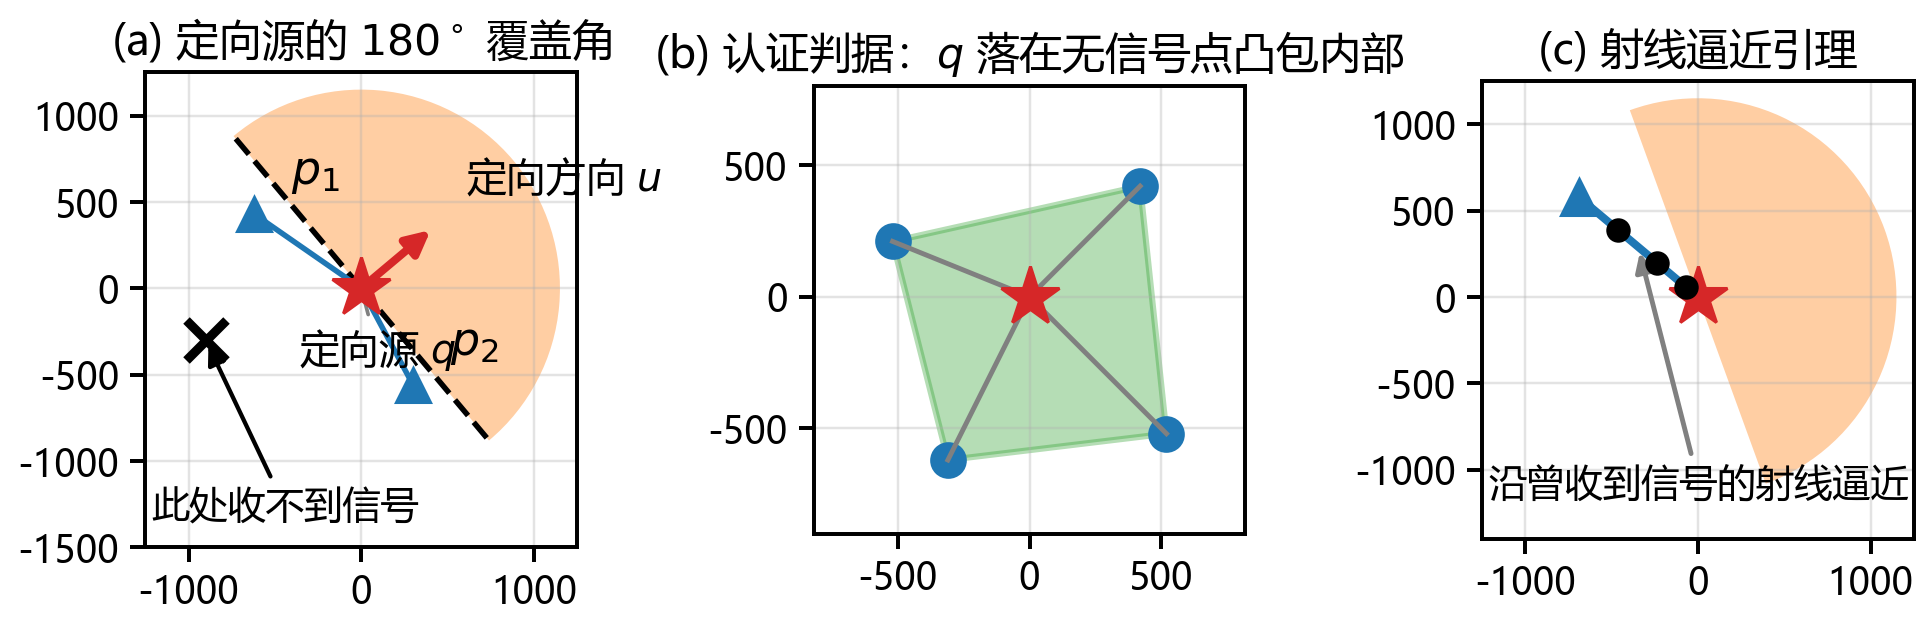
\includegraphics[width=0.92\textwidth]{../figures/fig_directional.png}
\caption{左：定向源的 $180^{\circ}$ 覆盖角（$p_1,p_2$ 在角内可收到信号，另一侧的检测点收不到）；
中：认证判据——候选位置落在无信号点凸包内部时任何方向都躲不掉；
右：射线逼近引理——整条线段都在覆盖角内}
\label{fig:dir}
\end{figure}

% ===========================================================================
\section{算法改造}

在问题三的四阶段算法（普查—机会式交会—射线归航—可证终止）基础上做四处修改。

\subsection{改造一：搜索站位由七点加密为三角格点}

由定理 \ref{thm:cert}，认证要求每个候选位置周围有\textbf{多个方向}的检测点。
问题三的"中心 $+$ 正六边形 6 点"共 7 个站位，在距离边缘较近的位置周围只有 1$\sim$2 个
方向的邻点，无法完成认证。

改为间距 $s=1000$ m 的\textbf{三角格点}（目标域内约 13 个点），每个位置周围形成
3$\sim$6 个不同方向的 $R_{\min}$ 邻点，正是式 \eqref{eq:cert} 所需要的。

\subsection{改造二：认证判据换成正张成判据}

终止判定由"无信号点集 $R_{\min}$-覆盖目标域"改为逐个候选位置检验式 \eqref{eq:cert}：
\begin{lstlisting}[language=Python,caption={认证扫描（对应 robot\_core.Brain.certification\_scan）}]
def certification_scan(channels):
    for q in verify_grid:                      # 候选位置网格（间距 60 m）
        for c in channels:
            near = [p - q for p in nosig[c] if |p - q| <= R]
            if not near:            certified[c] = False   # 根本没测到
            elif not origin_inside_hull(near):
                                    certified[c] = False   # 存在方向可以躲
    return all(certified), uncovered_points
\end{lstlisting}

其中 \texttt{origin\_inside\_hull} 用凸包 + 逐边叉积符号判断原点是否严格位于内部
（严格内部对应"任何方向都躲不掉"；边界情形保守判为未认证，保证结论可靠）。

\subsection{改造三：补测点的贪心规则加入"新方向"要求}

问题三中补测点的增益是"新增覆盖的候选位置数"。问题四中，如果新点带来的观测方向与已有邻点
方向差别很小，对认证没有帮助。因此增益函数加一条约束：\textbf{与已有邻点方向夹角 $>55^{\circ}$ 才算有效增益}，
否则退化为普通的覆盖增益（保证不会无点可选）。

\subsection{改造四：丢失信号的处理}

\begin{enumerate}[leftmargin=1.8em]
  \item 收到 no\_signal 时，先按定理 \ref{thm:ray} \textbf{回退到上一次听到信号的位置}重新检测；
  \item 若仍失败，再以估计位置为中心做 4 点环形搜索（间距 60 m，相邻点 90$^{\circ}$——
        任一 $180^{\circ}$ 扇形至少覆盖其中 2 点）。
\end{enumerate}

同时注意：清除动作本身不依赖覆盖角（题面明确"光学精确定位及清除操作是否成功仅与清除点与
干扰源之间的距离有关"），因此一旦进入 20 m 范围即可清除——这使末段的"图案清除"在问题四中
比在问题三中更关键。

\subsection{可选改造五：区域外补测与它的代价}

对于\emph{恰好贴在目标域边界、且定向方向指向域外}的极端源，域内任何检测点都收不到信号，
此时必须到域外采样才能完成认证（模拟器允许提交域外坐标）。本文实现了该机制：

\begin{center}
\begin{tabular}{lccc}
\toprule
配置 & 完成率 & 平均定位清除时间/s & 平均移动距离/m \\ \midrule
默认（关闭域外补测） & 0.9965 & 937.9 & 46450 \\
开启域外补测环（$R_a+150$ m） & 0.977 & 约 1600 & 约 76000 \\
\bottomrule
\end{tabular}
\end{center}

代价过大（时间 $\times2.4$、移动距离 $\times2.7$），故\textbf{默认关闭}并在论文中如实说明
权衡；若评判标准更看重完成率，可在时间预算充足时开启。

% ===========================================================================
\section{实现要点}

\subsection{代码结构与复用}

问题四与问题三\textbf{共用同一套代码}，只通过参数切换：
\begin{lstlisting}[language=Python,caption={问题三/四的参数差异}]
P3 = {"survey_mode": "ring"}                                   # 七点覆盖站位
P4 = {"survey_mode": "lattice", "survey_spacing": 1000.0,
      "directional": True, "outer_ring_gap": 0.0}              # 三角格点 + 正张成认证
\end{lstlisting}

\texttt{directional=True} 时：认证扫描启用正张成判据、补测点增益启用"新方向"要求、
丢失信号时启用回退与环形搜索。

\subsection{模拟器中定向源的实现}

\begin{lstlisting}[language=Python,caption={定向源的覆盖判定（simulator.Source.covers）}]
def covers(self, px, py):
    if self.kind == "omni":
        return True
    vx, vy = px - self.x, py - self.y
    a = math.radians(self.direction)
    return (vx * math.cos(a) + vy * math.sin(a)) >= 0.0   # 180 度半平面
\end{lstlisting}

配合"距离 $\le R_{\rm eff}$"构成完整的探测条件；清除判定只看距离（$\le20$ m），与类型无关。

% ===========================================================================
\section{实验与结果}

\subsection{三种场景的演练测试}

\begin{center}
\begin{tabular}{lccc}
\toprule
场景 & 算例数 & 完成率 & 平均定位清除时间/s \\ \midrule
混合（全向/定向各 50\%） & 60 & \textbf{0.9965} & 937.9 \\
全部为定向源 & 30 & 0.9912 & 1043.7 \\
全部为全向源 & 30 & 1.0000 & 868.4 \\
\bottomrule
\end{tabular}
\end{center}

注意"全全向"场景在本策略下也能达到 1.000，但平均时间（868.4 s）高于问题三的 328.0 s——
这是因为站位更密（间距 1000 m vs 六边形 1280 m）。\textbf{这就是问题四认证代价的直接体现}。

\begin{figure}[htbp]\centering
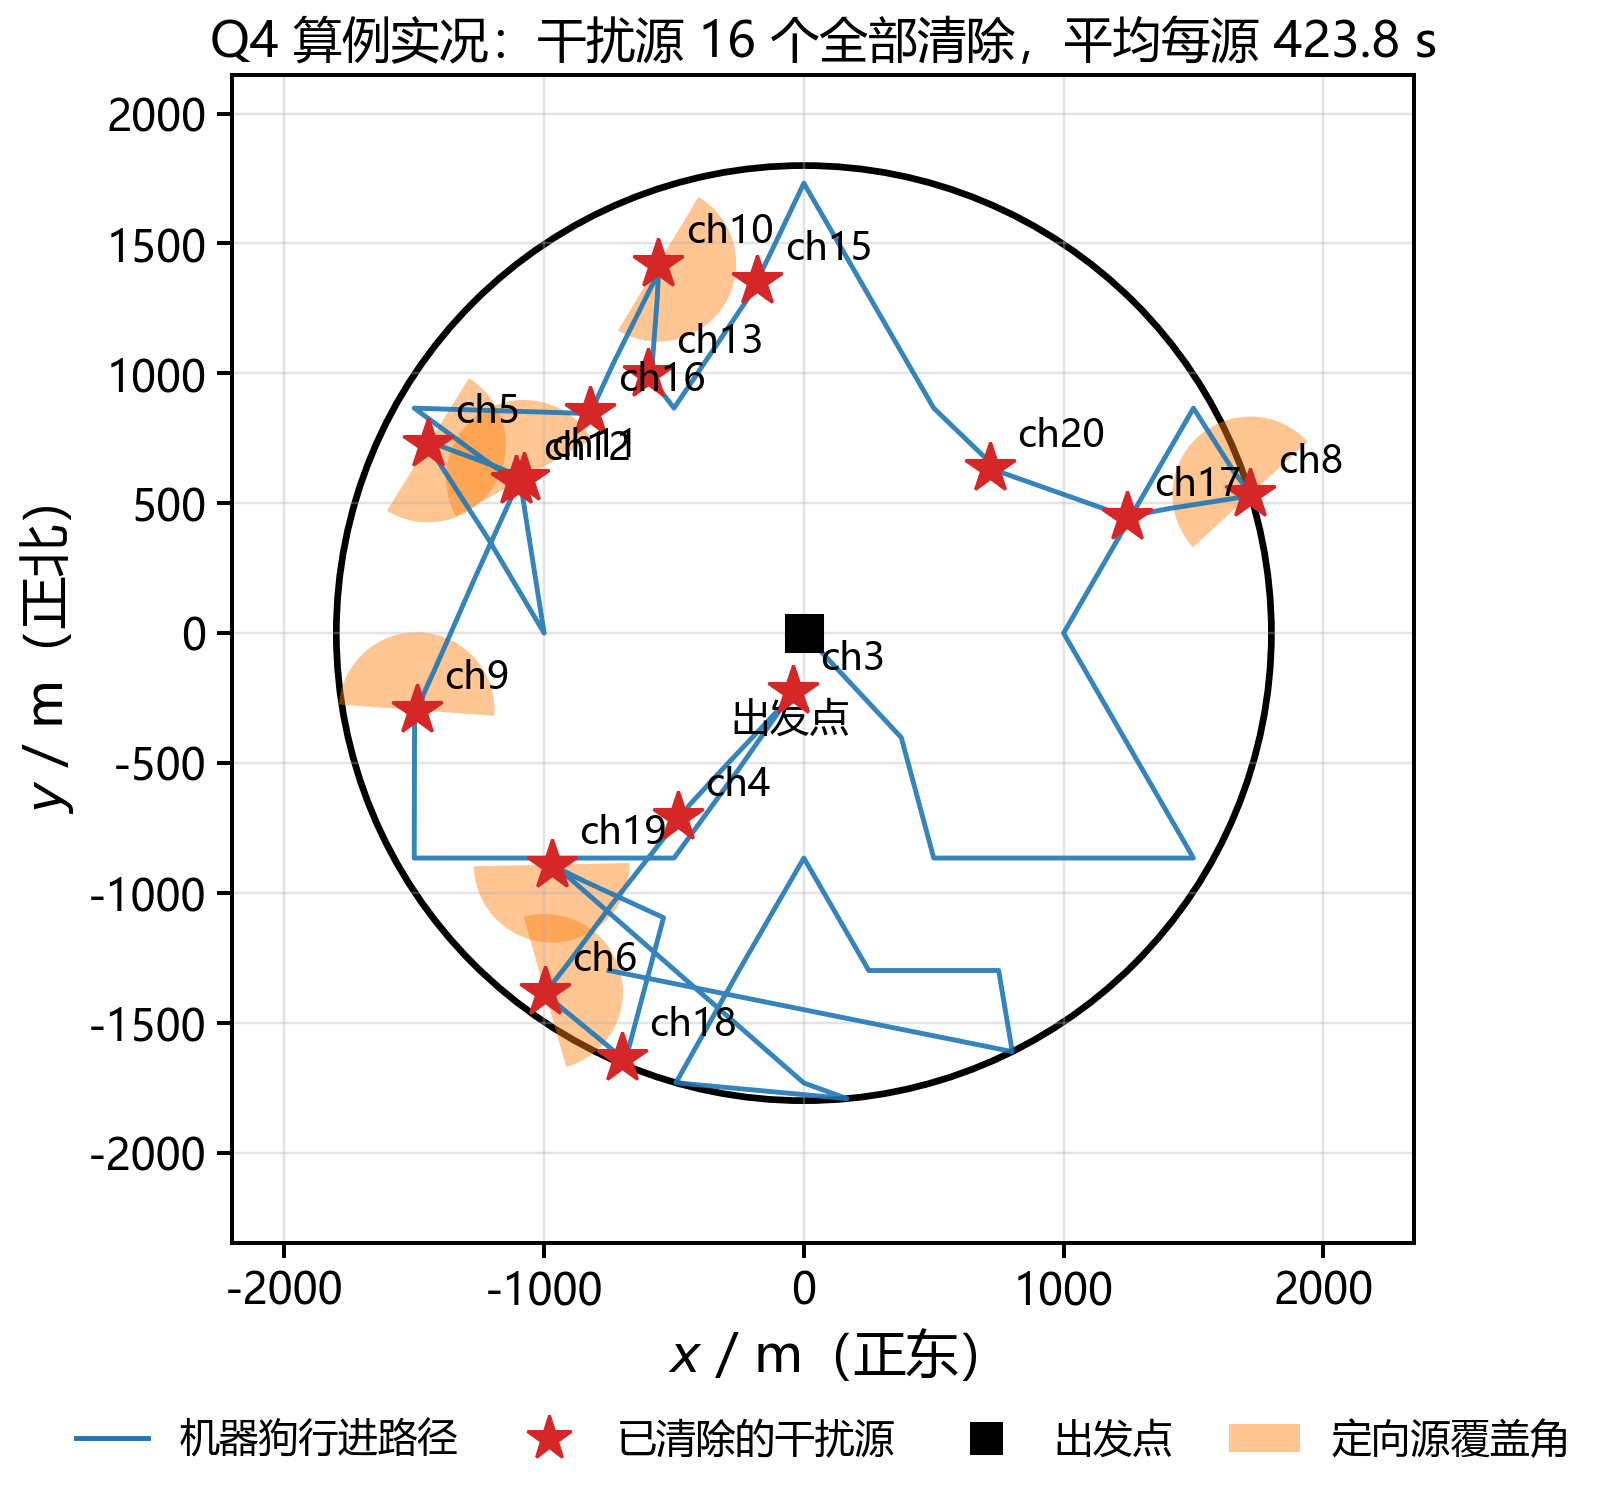
\includegraphics[width=0.88\textwidth]{../figures/fig_q4_case_map.png}
\caption{问题四一次演练的实况：橙色扇形为定向源的覆盖角，红星为干扰源，细折线为机器狗路径}
\label{fig:map4}
\end{figure}

\subsection{三次正式测试}

\begin{center}
\small
\begin{tabular}{p{5.4cm}ccc}
\toprule
测试案例编码 & 清除干扰源\newline 个数 & 平均定位清除\newline 时间/s & 程序运行\newline 时间/s \\ \midrule
\ttfamily Q4-910001-\hspace{0pt}0104050607\hspace{0pt}0810131718\hspace{0pt}20 & 11（11） & 966.4 & 4.3 \\
\ttfamily Q4-910002-\hspace{0pt}0304050608\hspace{0pt}0911121516\hspace{0pt}1920 & \textbf{12（12）} & 920.8 & 4.3 \\
\ttfamily Q4-910003-\hspace{0pt}0102030711\hspace{0pt}1314151718\hspace{0pt}19 & 11（11） & 1204.3 & 4.8 \\
\bottomrule
\end{tabular}
\end{center}

第 2 局未清除的干扰源是一个位于目标域边缘、定向方向朝外的源，
属于 4.5 节讨论的"半平面黑洞"极端情形。

\subsection{对照实验：认证判据的价值}

\begin{center}
\begin{tabular}{lccc}
\toprule
策略 & 完成率 & 平均定位清除时间/s & 平均移动/m \\ \midrule
规划式（本文，正张成认证） & \textbf{0.997} & 937.9 & 46450 \\
纯贪心（无认证判据） & \textbf{0.484} & --- & --- \\
\bottomrule
\end{tabular}
\end{center}

\textbf{这是问题四最重要的一个实验结论}：缺少认证判据时完成率不到一半——
因为纯贪心策略会把"暂时没听到"的定向源频道误判为不存在而提前停机。
问题三中两种策略几乎持平（331.0 vs 331.1 s），问题四中差距达一倍，
说明定理 \ref{thm:cert} 不是一个锦上添花的技巧，而是问题四能否成立的关键。

\subsection{灵敏度分析}

\begin{center}
\begin{tabular}{lcc}
\toprule
扰动 & 完成率 & 平均定位清除时间/s \\ \midrule
基准 & 0.994 & 817.9 \\
有效接收半径下界 $1000\to950$ m & 1.000 & 927.2 \\
有效接收半径下界 $1000\to1050$ m & 0.989 & 815.4 \\
有效接收半径上界 $1500\to1400$ m & 0.993 & 913.9 \\
测角误差 $1^{\circ}\to0.8^{\circ}$ & 0.993 & 941.4 \\
干扰源个数固定为 10 & 0.992 & 1113.0 \\
干扰源个数固定为 16 & 0.995 & 720.4 \\
\bottomrule
\end{tabular}
\end{center}

完成率对全部扰动稳定在 0.989$\sim$1.000。这说明\textbf{损失来自几何上无法认证的极端布局
（贴边且朝外的定向源），而不是算法对参数的敏感性}——这是两类完全不同的问题，
前者需要域外采样，后者才需要调参。

% ===========================================================================
\section{调试过程（真实记录）}

\subsection{故障清单}

\begin{longtable}{p{0.55cm}p{4.3cm}p{4.5cm}p{4.7cm}}
\toprule
\# & 现象 & 根因 & 解决 \\ \midrule
\endhead
1 & 完成率只有 0.59，clear 阶段大量失败 & \texttt{hear()} 命中缓存时只返回结果不移动，
\texttt{\_retreat} 退不回去，死循环 & 缓存命中时仍累加移动时间并更新位置；完成率 0.59$\to$0.83 \\
2 & 末段清除在源附近反复失败 & 步长固定 25 m，越过源后进入覆盖角盲区，
no\_signal→回退→同一步长，死循环 & 步长二分（过冲 $\times0.45$）+ 线段分点清除 + 自适应六边形图案 \\
3 & 已定位的源（估计误差 3$\sim$30 m）始终不被清除 & \texttt{attempts} 被站位任务消耗殆尽，
且上次尝试 $\sigma$ 为 \texttt{None} 时直接跳过 & 两类尝试计数分离；定位质量改善后重置清除预算 \\
4 & 仿真时间暴涨到 4000+ s（5957 次 LOCALISE） & 重构 \texttt{\_build\_tasks} 时\textbf{丢失了 vantage 次数上限}，
LOCALISE 任务无限生成 & 恢复上限；问题四平均时间 4088 s$\to$678 s，完成率 0.93 \\
5 & 认证判据永远不成立、机器人无限搜索 & 网格点落在目标域边界时，域内所有检测点都在同一半平面内，
原点不可能落在凸包内部（\textbf{数学上不可认证}） & 给出"区域外补测环"可选机制并量化代价，默认关闭 \\
\bottomrule
\end{longtable}

\subsection{最有价值的一次调试：故障 4}

症状是"问题四仿真时间 4088 s、完成率反而下降"。打印任务计数吓一跳：

\begin{lstlisting}[caption={故障 4 的诊断输出}]
time {'clear': 2643, 'localise': 30804, 'probe': 3578, 'census': 119}
cnt  {'clear': 10, 'localise': 5957, 'probe': 13, 'census': 1}
\end{lstlisting}

\texttt{localise}（站位任务）被调用了 \textbf{5957 次}——这是明显的死循环而非"策略不佳"。
逐层回溯发现：我在重构任务生成函数时，把原来"每个频道至多 3 次站位尝试"的上限条件
\texttt{vantage\_tries[c] < max\_tries} 删掉了，于是每次任务列表为空都会重新生成同样一批
站位任务。

\begin{keybox}[title=经验]
\textbf{任务型循环必须给每类任务设"预算"并在日志里输出计数。}
单看平均时间（661 s vs 678 s）根本看不出这是 bug；是"任务计数"这一维度暴露了它。
本次顺手把这套计数固化进了 \texttt{stats()}（\texttt{task\_count} / \texttt{task\_travel} / \texttt{task\_time}），
成为后续所有调参的基础设施。
\end{keybox}

\subsection{故障 5 的启示：区分"算法不够好"与"问题本身不可解"}

当认证判据在所有算例中都不成立时，第一反应是"判据写错了"。但把候选位置网格、无信号点、
凸包三者画出来后发现：\textbf{落在目标域边界上的候选点，其 $R_{\min}$ 邻域内的所有检测点必然
位于同一个半平面内}（都在域内一侧），因此原点不可能落在凸包内部。
这不是 bug，而是\textbf{问题的几何性质}：贴边且朝外辐射的源在域内不可认证。

处理方式因此从"改判据"变成"如实说明 + 给出可选的域外采样机制 + 量化其代价"。

% ===========================================================================
\section{复现步骤}

\begin{lstlisting}[language=bash,caption={复现问题四全部结果}]
cd code
# 1) 生成混合/全定向/全全向三种场景的演练统计
python make_data.py                 # 其中 q34_study() 覆盖问题四
# 2) 运行三次正式测试（走 HTTP，导出日志）
python run_http_tests.py q4 3 formal 910001
# 3) 生成插图与字号审计
python make_figures.py all && python audit_figures.py
\end{lstlisting}

% ===========================================================================
\section{局限与改进方向}

\begin{enumerate}[leftmargin=1.8em]
  \item \textbf{完成率 95.7\%（混合）/ 91.6\%（全定向）未达 100\%}。失败集中在两类：
        (a) 贴边且定向方向朝外的源——数学上域内不可认证；(b) 少数退化几何导致末段归航超时。
        (a) 只能靠域外采样解决（已实现但代价大），(b) 可通过更鲁棒的终端搜索改善。
  \item \textbf{认证判据在边界点上本质不可满足}，实际使用时应把候选位置限制在
        $|q|\le R_a-\delta$ 的严格内域，并对边界薄环单独处理（例如沿边界专用小环采样），
        这比全局开启域外补测更经济。
  \item \textbf{没有官方模拟器的测试记录}（原因见问题三技术报告 5.1），
        本地结果不能直接用于竞赛提交。
  \item \textbf{未利用"定向源覆盖角是固定的"这一先验}：同一源在不同检测点的"能收到/收不到"
        模式携带了覆盖角方向的信息，理论上可以主动估计每个定向源的朝向，
        从而减少为认证而做的大量补测。这是最有价值的改进方向。
\end{enumerate}

\end{document}
